\chapter{Transducer (2012)}

\begin{tcolorbox}
\fullcite{arxiv/1211.3711/Sequence-Transduction-RNN}
\end{tcolorbox}



\begin{enumerate}
    \item Many machine learning tasks can be expressed as the transformation—or transduction—of input sequences into output sequences. 
    Example: speech recognition, machine translation, protein secondary structure prediction and text-to-speech, etc
    \hfill \cite{arxiv/1211.3711/Sequence-Transduction-RNN}

    \item One of the key challenges in sequence transduction is learning to represent both the input and output sequences in a way that is \textbf{invariant to sequential distortions} such as shrinking, stretching and translating.
    \hfill \cite{arxiv/1211.3711/Sequence-Transduction-RNN}

    \item For a general-purpose sequence transducer, where the output length is \textbf{unknown} in advance, we would prefer a distribution over sequences of \textbf{all} lengths.
    Furthermore, since we do not know how the inputs and outputs should be aligned, this distribution would ideally cover all possible alignments.
    \hfill \cite{arxiv/1211.3711/Sequence-Transduction-RNN}

    \item The transducer extends CTC by defining a distribution over output sequences of all lengths, and by jointly modelling both input-output and output-output dependencies.
    \hfill \cite{arxiv/1211.3711/Sequence-Transduction-RNN}

    \item As a discriminative sequential model the transducer has similarities with ‘chain-graph’ conditional random fields (CRFs).
    However the transducer’s construction from RNNs, with their ability to extract features from raw data and their potentially unbounded range of dependency, is in marked contrast with the pairwise output potentials and hand-crafted input features typically used for CRFs.
    \hfill \cite{arxiv/1211.3711/Sequence-Transduction-RNN}

    \item Transducer is closer in spirit is the \textbf{Graph Transformer Network} paradigm, in which differentiable modules (often neural networks) can be globally trained to perform consecutive graph transformations such as detection, segmentation and recognition.
    \hfill \cite{arxiv/1211.3711/Sequence-Transduction-RNN}
\end{enumerate}




\section{RNN Transducer}

\begin{enumerate}
    \item Let $\bm{x} = (x_1, x_2, \cdots , x_T )$ be a length $T$ input sequence of arbitrary length belonging to the set $X ^\ast$ of all sequences over some input space $X $.
    Let $\bm{y} = (y_1, y_2, \cdots , y_U )$ be a length $U$ output sequence belonging to the set $Y^\ast$ of all sequences over some output space $Y$. 
    We assume that the output space is discrete; however the method can be readily extended to continuous output spaces, provided a tractable, differentiable model can be found for $Y$.
    \hfill \cite{arxiv/1211.3711/Sequence-Transduction-RNN}

    \item Both the inputs vectors $x_t$ and the output vectors $y_u$ are represented by fixed-length real-valued vectors; 
    \hfill \cite{arxiv/1211.3711/Sequence-Transduction-RNN}

    \item Let the extended output space $\bar{Y} = Y \cup \varnothing$, where $\varnothing$ denotes the \textbf{null output}. 
    The intuitive meaning of $\varnothing$ is ‘output nothing’; the sequence $(y_1, \varnothing, \varnothing, y_2, \varnothing, y_3) \in \bar{Y}^\ast$ is therefore equivalent to $(y_1, y_2, y_3) \in Y^\ast$.
    \hfill \cite{arxiv/1211.3711/Sequence-Transduction-RNN}

    \item We refer to the elements $a \in \bar{Y}^\ast$ as alignments, since the location of the null symbols determines an alignment between the input and output sequences. 
    \hfill \cite{arxiv/1211.3711/Sequence-Transduction-RNN}

    \item Given $x$, the RNN transducer defines a conditional distribution $P(a \in \bar{Y}^\ast|x)$.
    This distribution is then collapsed onto the following distribution over ${Y}^\ast$:
    \hfill \cite{arxiv/1211.3711/Sequence-Transduction-RNN}
    \\[0.2cm]
    .\hfill
    $
        P(y\in Y^\ast|x) = \dsum_{a \in B^{-1}(y)} P(a|x)
    $
    \hfill \cite{arxiv/1211.3711/Sequence-Transduction-RNN}
    \\[0.2cm]
    where $B : \bar{Y}^\ast \mapsto Y^\ast$ is a function that removes the null symbols from the alignments in $\bar{Y}^\ast$.
    \hfill \cite{arxiv/1211.3711/Sequence-Transduction-RNN}

    \item Two recurrent neural networks are used to determine $P(a \in \bar{Y}^\ast|x)$.
    \hfill \cite{arxiv/1211.3711/Sequence-Transduction-RNN}
    \begin{enumerate}
        \item \textbf{transcription network} $F$: scans the input sequence $x$ and outputs the sequence $\bm{f} = (f_1, \cdots , f_T )$ of transcription vectors.
        \hfill \cite{arxiv/1211.3711/Sequence-Transduction-RNN}

        \item The other network, referred to as the prediction network $G$, scans the output sequence $\bm{y}$ and outputs the prediction vector sequence $\bm{g} = (g_0, g_1, \cdots , g_U )$.
        \hfill \cite{arxiv/1211.3711/Sequence-Transduction-RNN}
    \end{enumerate}

    \item  For a task with $K$ output labels, the output layer of the transcription network is size $K + 1$, just like the prediction network, and hence the transcription vectors $f_t$ are also size $K + 1$.
    \hfill \cite{arxiv/1211.3711/Sequence-Transduction-RNN}
\end{enumerate}


\subsection{Prediction Network ($G$)}

\begin{enumerate}
    \item The prediction network $G$ is a recurrent neural network consisting of an input layer, an output layer and a single hidden layer.
    The length $U + 1$ input sequence $\hat{\bm{y}} = (\varnothing, y_1, \cdots , y_U )$ to $G$ output sequence $\bm{y}$ with $\varnothing$ prepended. 
    \hfill \cite{arxiv/1211.3711/Sequence-Transduction-RNN}
    
    \item The inputs are encoded as one-hot vectors; that is, if $Y$ consists of $K$ labels and $y_u = k$, then $\hat{\bm{y}}_u$ is a length $K$ vector whose elements are all zero except the $k$-th, which is one. 
    $\varnothing$ is encoded as a length $K$ vector of zeros.
    The input layer is therefore size $K$. 
    \hfill \cite{arxiv/1211.3711/Sequence-Transduction-RNN}

    \item The output layer is size $K + 1$ (one unit for each element of $\bar{Y}$) and hence the prediction vectors $g_u$ are also size $K + 1$.
    \hfill \cite{arxiv/1211.3711/Sequence-Transduction-RNN}

    \item Given $\hat{\bm{y}}$, $G$ computes the hidden vector sequence $(h_0, \cdots , h_U )$ and the prediction sequence $(g_0, \cdots , g_U )$ by iterating the following equations from $u = 0$ to $U $:
    \hfill \cite{arxiv/1211.3711/Sequence-Transduction-RNN}
    \begin{multicols}{2}
    \begin{enumerate}
        \item $h_u = H (W_{ih} \hat{\bm{y}}_u + W_{hh}h_{u-1} + b_h)$
        \hfill \cite{arxiv/1211.3711/Sequence-Transduction-RNN}

        \item $g_u = W_{ho}h_u + b_o $
        \hfill \cite{arxiv/1211.3711/Sequence-Transduction-RNN}
    \end{enumerate}
    \end{multicols}
    where $W_{ih}$ is the input-hidden weight matrix, 
    $W_{hh}$ is the hidden-hidden weight matrix, 
    $W_{ho}$ is the hidden-output weight matrix, 
    $b_h$ and $b_o$ are bias terms, 
    and $H$ is the hidden layer function. 
    \hfill \cite{arxiv/1211.3711/Sequence-Transduction-RNN}

    \item In traditional RNNs $H$ is an elementwise application of the $\tanh$ or logistic sigmoid $\sigma(x) = \dfrac{1}{1 + \exp(-x)}$ functions.
    \hfill \cite{arxiv/1211.3711/Sequence-Transduction-RNN}

    \item The prediction network attempts to model each element of $\bm{y}$ given the previous ones; it is therefore similar to a standard next-step-prediction RNN, only with the added option of making ‘null’ predictions.
    \hfill \cite{arxiv/1211.3711/Sequence-Transduction-RNN}
\end{enumerate}


\subsection{Transcription Network ($F$)}


\begin{enumerate}
    \item The transcription network $F$ is a bidirectional RNN that scans the input sequence $\bm{x}$ forwards and backwards with two separate hidden layers, both of which feed forward to a single output layer. 
    \hfill \cite{arxiv/1211.3711/Sequence-Transduction-RNN}

    \item Bidirectional RNNs are preferred because each output vector depends on the whole input sequence (rather than on the previous inputs only, as is the case with normal RNNs).
    \hfill \cite{arxiv/1211.3711/Sequence-Transduction-RNN}

    \item Given a length $T$ input sequence $(x_1 \cdots x_T )$, a bidirectional RNN computes the forward hidden sequence $(\overrightarrow{h_1}, \cdots , \overrightarrow{h_T} )$, the backward hidden sequence $(\overleftarrow{h_1}, \cdots , \overleftarrow{h_T} )$, and the transcription sequence $(f_1, \cdots , f_T )$ by first iterating the backward layer from $t = T$ to $1$:
    \hfill \cite{arxiv/1211.3711/Sequence-Transduction-RNN}
    \\[0.2cm]
    .\hfill
    $\overleftarrow{h}_ t = H\dParenBrac{W_{i\overleftarrow{h}} i_t + W_{\overleftarrow{h} \overleftarrow{h}} \overleftarrow{h} _{t+1} + b_{\overleftarrow{h}}}$
    \hfill \cite{arxiv/1211.3711/Sequence-Transduction-RNN}
    
    
    \item iterating the forward and output layers from $t = 1$ to $T $:
    \hfill \cite{arxiv/1211.3711/Sequence-Transduction-RNN}
    \\[0.2cm]
    .\hfill
    $\overrightarrow{h}_ t = H\dParenBrac{W_{i\overrightarrow{h}} i_t + W_{\overrightarrow{h} \overrightarrow{h}} \overrightarrow{h} _{t+1} + b_{\overrightarrow{h}}}$
    \hfill \cite{arxiv/1211.3711/Sequence-Transduction-RNN}

    \item $o_t = W_{\overrightarrow{h} o} \overrightarrow{h}_ t + W_{\overleftarrow{h} o}\overleftarrow{h}_ t + b_o $
    \hfill \cite{arxiv/1211.3711/Sequence-Transduction-RNN}

    \item The transcription network is similar to a Connectionist Temporal Classification RNN, which also uses a null output to define a distribution over input-output alignments.
    \hfill \cite{arxiv/1211.3711/Sequence-Transduction-RNN}
\end{enumerate}



\subsection{Output Distribution}

\begin{table}[H]
\begin{minipage}{0.3\linewidth}
\begin{figure}[H]
    \centering
    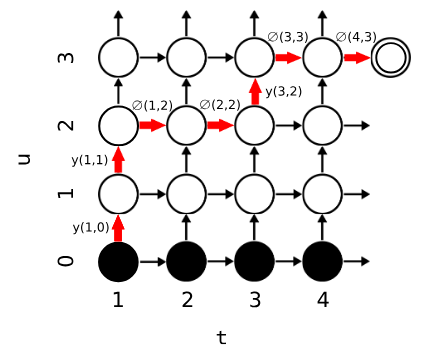
\includegraphics[
        width=\linewidth,
        height=6cm,
        keepaspectratio,
    ]{images/advanced-ml/arxiv-1211.3711v1.fig-1-output-lattice.png}
\end{figure}
\end{minipage}
\hfill
\begin{minipage}{0.65\linewidth}
\begin{enumerate}
    \item Output probability lattice defined by $P(k|t, u)$. 
    \hfill \cite{arxiv/1211.3711/Sequence-Transduction-RNN}
    
    \item The \textbf{node} at $(t, u)$ represents the probability of having output the first $u$ elements of the output sequence by point $t$ in the transcription sequence. 
    \hfill \cite{arxiv/1211.3711/Sequence-Transduction-RNN}
    
    \item The \textbf{horizontal arrow} leaving node $(t, u)$ represents the probability $\varnothing(t, u)$ of outputting nothing at $(t, u)$; 
    the \textbf{vertical arrow} represents the probability $y(t, u)$ of outputting the element $u + 1$ of $\bm{y}$. 
    \hfill \cite{arxiv/1211.3711/Sequence-Transduction-RNN}
    
    \item The \textbf{black nodes} at the bottom represent the null state before any outputs have been emitted. 
    \hfill \cite{arxiv/1211.3711/Sequence-Transduction-RNN}
    
    \item The \textbf{paths} starting at the bottom left and reaching the terminal node in the top right (one of which is shown in red) correspond to the possible alignments between the input and output sequences. 
    \hfill \cite{arxiv/1211.3711/Sequence-Transduction-RNN}
    
    \item Each alignment starts with probability 1, and its final probability is the product of the transition probabilities of the arrows they pass through (shown for the red path).
    \hfill \cite{arxiv/1211.3711/Sequence-Transduction-RNN}
\end{enumerate}
\end{minipage}
\end{table}


\begin{enumerate}
    \item Given the transcription vector $f_t$, where $1 leq t leq T $, the prediction vector $g_u$, where $0 leq u leq U $, and label $k \in \bar{Y}$, define the \textbf{output density function}:
    \colorbox{yellow}{$h(k, t, u) = \exp (f ^k _t + g^k _u ) $}
    where superscript $k$ denotes the $k$-th element of the vectors. 
    \hfill \cite{arxiv/1211.3711/Sequence-Transduction-RNN}

    \item The density can be normalised to yield the conditional output distribution:
    \colorbox{yellow}{$P(k \in \bar{Y}|t, u) = \dfrac{h(k, t, u)}{\tsum_{k^\prime \in \bar{Y}} h(k^\prime, t, u)}$}
    \hfill \cite{arxiv/1211.3711/Sequence-Transduction-RNN}

    \item simply: 
    \hfill
    $ y(t, u) \equiv P(y_{u+1}|t, u) $
    \hfill
    $ \varnothing(t, u) \equiv P(\varnothing|t, u) $
    \hfill \cite{arxiv/1211.3711/Sequence-Transduction-RNN}

    \item $P(k|t, u)$ is used to determine the transition probabilities in the lattice.
    \hfill \cite{arxiv/1211.3711/Sequence-Transduction-RNN}

    \item The set of possible paths from the start node to the terminal node corresponds to the complete set of alignments between $\bm{x}$ and $\bm{y}$, i.e. to the set $\bar{Y}^\ast \cap B^{-1}(\bm{y})$. 
    Therefore all possible input-output alignments are assigned a probability, the sum of which is the total probability $P(\bm{y}|\bm{x})$ of the output sequence given the input sequence.
    \hfill \cite{arxiv/1211.3711/Sequence-Transduction-RNN}

    \item Since a similar lattice could be drawn for any finite $\bm{y} \in Y^\ast$, $P(k|t, u)$ defines a distribution over all possible output sequences, given a single input sequence.
    \hfill \cite{arxiv/1211.3711/Sequence-Transduction-RNN}
\end{enumerate}



\section{LSTM Transducer}

\subsection{Prediction Network ($G$)}

\begin{enumerate}
    \item we have found that the Long Short-Term Memory (LSTM) architecture is better at finding and exploiting long range contextual information.
    \hfill \cite{arxiv/1211.3711/Sequence-Transduction-RNN}

    \item hidden layer function $H$ is implemented by the following composite function:
    \begin{multicols}{2}
    \begin{enumerate}
        \item $\alpha _n = \sigma  (W_{i\alpha }i_n + W_{h\alpha }h_{n-1} + W_{s\alpha }s_{n-1})$
        \hfill \cite{arxiv/1211.3711/Sequence-Transduction-RNN}

        \item $\beta _n = \sigma  (W_{i\beta } i_n + W_{h\beta } h_{n-1} + W_{s\beta } s_{n-1})$
        \hfill \cite{arxiv/1211.3711/Sequence-Transduction-RNN}

        \item $s_n = \beta _ns_{n-1} + \alpha _n \tanh (W_{is}i_n + W_{hs}) $
        \hfill \cite{arxiv/1211.3711/Sequence-Transduction-RNN}

        \item $\gamma _n = \sigma  (W_{i\gamma } i_n + W_{h\gamma } h_{n-1} + W_{s\gamma } s_n)$
        \hfill \cite{arxiv/1211.3711/Sequence-Transduction-RNN}

        \item $h_n = \gamma _n \tanh(s_n) $
        \hfill \cite{arxiv/1211.3711/Sequence-Transduction-RNN}
    \end{enumerate}
    \end{multicols}
    where $\alpha, \beta, \gamma$ and $s$ are respectively the \textbf{input gate, forget gate, output gate} and \textbf{state vectors}, all of which are the same size as the hidden vector $h$. 
    \item $W_{h\alpha}$ is the hidden-input gate matrix, $W{i\gamma}$ is the input-output gate matrix etc.
    \hfill \cite{arxiv/1211.3711/Sequence-Transduction-RNN}

    \item The weight matrices from the state to gate vectors are diagonal, so element $m$ in each gate vector only receives input from element $m$ of the state vector. 
    The bias terms (which are added to $\alpha, \beta, s$ and $\gamma$) have been omitted for clarity.
    \hfill \cite{arxiv/1211.3711/Sequence-Transduction-RNN}

    \item 
\end{enumerate}








\section{Forward-Backward Algorithm}

\begin{enumerate}
    \item Define the forward variable $\alpha(t, u)$ as the probability of outputting $\bm{y}_{[1:u]}$ during $\bm{f}_{[1:t]}$.
    \hfill \cite{arxiv/1211.3711/Sequence-Transduction-RNN}

    \item The forward variables for all $1 \leq t \leq T$ and $0 \leq u \leq U$ can be calculated recursively using:
    \hfill \cite{arxiv/1211.3711/Sequence-Transduction-RNN}
    \\[0.2cm]
    .\hfill
    $\alpha(t, u) = \alpha(t - 1, u)\varnothing(t - 1, u) + \alpha(t, u - 1)y(t, u - 1)$
    \hfill \cite{arxiv/1211.3711/Sequence-Transduction-RNN}
    \\[0.2cm]
    with initial condition $\alpha(1, 0) = 1$.
    \hfill \cite{arxiv/1211.3711/Sequence-Transduction-RNN}

    \item The total output sequence probability is equal to the forward variable at the terminal node:
    \hfill \cite{arxiv/1211.3711/Sequence-Transduction-RNN}
    \\[0.2cm]
    .\hfill
    $P(\bm{y}|x) = \alpha(T, U )\varnothing(T, U )$
    \hfill \cite{arxiv/1211.3711/Sequence-Transduction-RNN}

    \item Define the backward variable $\beta(t, u)$ as the probability of outputting $\bm{y}_{[u+1:U ]}$ during $\bm{f}_{[t:T ]}$.
    \hfill \cite{arxiv/1211.3711/Sequence-Transduction-RNN}

    \item $\beta(t, u) = \beta(t + 1, u)\varnothing(t, u) + \beta(t, u + 1)y(t, u)$
    \hfill \cite{arxiv/1211.3711/Sequence-Transduction-RNN}
    \\[0.2cm]
    with initial condition $\beta(T, U ) = \varnothing(T, U )$. 
    \hfill \cite{arxiv/1211.3711/Sequence-Transduction-RNN}

    \item From the definition of the forward and backward variables it follows that their product $\alpha(t, u)\beta(t, u)$ at any point $(t, u)$ in the output lattice is equal to the probability of emitting the complete output sequence if $y_u$ is \textbf{emitted during transcription} step $t$. 
    \hfill \cite{arxiv/1211.3711/Sequence-Transduction-RNN}
\end{enumerate}


\section{Training}

\begin{enumerate}
    \item Given an input sequence $\bm{x}$ and a target sequence $\bm{y}^\ast$, the natural way to train the model is to minimise the log-loss $L = - \ln (P(\bm{y}^\ast|\bm{x}))$ of the target sequence.
    \hfill \cite{arxiv/1211.3711/Sequence-Transduction-RNN}

    \item $\forall n : 1 \leq n \leq U + T,\ P(\bm{y}^\ast|\bm{x}) = \dsum_{(t,u):t+u=n} \alpha(t, u)\beta(t, u) $
    \hfill \cite{arxiv/1211.3711/Sequence-Transduction-RNN}

    \item $
        \dfrac{\partial L}{\partial P(k|t, u)}
        = \dfrac{\alpha(t, u)}{P(\bm{y}^\ast|\bm{x})}
        = \begin{cases}
            \beta(t, u + 1) & \text{ if } k = y_{u+1} \\
            \beta(t + 1, u) & \text{ if } k = \varnothing \\
            0 & otherwise
        \end{cases}
    $
    \hfill \cite{arxiv/1211.3711/Sequence-Transduction-RNN}
    \begin{multicols}{2}
    \begin{enumerate}
        \item 
        $
            \dfrac{\partial L}{\partial f ^k_t} = 
            \dsum_{u=0}^U \dsum_{k^\prime \in \bar{Y}}
            \dfrac{\partial L}{\partial  Pr(k^\prime |t, u)} \dfrac{\partial  Pr(k^\prime |t, u)}{\partial f ^k_t}
        $
        \hfill \cite{arxiv/1211.3711/Sequence-Transduction-RNN}

        \item 
        $
            \dfrac{\partial L}{\partial g ^k_u} = 
            \dsum_{t=1}^T \dsum_{k^\prime \in \bar{Y}}
            \dfrac{\partial L}{\partial  Pr(k^\prime |t, u)} \dfrac{\partial  Pr(k^\prime |t, u)}{\partial g ^k_u}
        $
        \hfill \cite{arxiv/1211.3711/Sequence-Transduction-RNN}
    \end{enumerate}
    \end{multicols}
    where, 
    $
        \dfrac{\partial  Pr(k^\prime |t, u)}{\partial f ^k_t}
        = \dfrac{\partial  Pr(k^\prime |t, u)}{\partial g ^k_u}
        = P(k^\prime|t, u) [\delta_{kk^\prime} - P(k|t, u)]
    $
    \hfill \cite{arxiv/1211.3711/Sequence-Transduction-RNN}

    \item A separate softmax could be calculated for every $P(k|t, u)$ required by the forward-backward algorithm. 
    \hfill \cite{arxiv/1211.3711/Sequence-Transduction-RNN}
    \begin{enumerate}
        \item this is computationally expensive due to the high cost of the exponential function.
        \hfill \cite{arxiv/1211.3711/Sequence-Transduction-RNN}

        \item we can instead pre-compute all the $\exp (f (t, x))$ and $\exp(g(y_{[1:u]}))$ terms and use their products to determine $P(k|t, u)$. 
        \hfill \cite{arxiv/1211.3711/Sequence-Transduction-RNN}

        \item This reduces the number of exponential evaluations from $\mathcal{O}(T U )$ to $\mathcal{O}(T + U )$ for each length $T$ transcription sequence and length $U$ target sequence used for training.
        \hfill \cite{arxiv/1211.3711/Sequence-Transduction-RNN}
    \end{enumerate}
\end{enumerate}



\section{Testing/ Inference}

\begin{enumerate}
    \item When the transducer is evaluated on test data, we seek the mode of the output sequence distribution induced by the input sequence.
    \hfill \cite{arxiv/1211.3711/Sequence-Transduction-RNN}

    \item Unfortunately, finding the mode is much harder than determining the probability of a single sequence. 
    The complication is that the prediction function $g(y_{[1:u]})$ (and hence the output distribution $P(k|t, u))$ may depend on all previous outputs emitted by the model.
    \hfill \cite{arxiv/1211.3711/Sequence-Transduction-RNN}

    \item The method employed is a fixed-width beam search through the tree of output sequences. 
    The advantage of beam search is that it scales to arbitrarily long sequences, and allows computational cost to be traded off against search accuracy.
    \hfill \cite{arxiv/1211.3711/Sequence-Transduction-RNN}

    \item Let $P(\bm{y})$ be the approximate probability of emitting some output sequence $\bm{y}$ found by the search so far.
    Let $P(k|\bm{y}, t)$ be the probability of extending $\bm{y}$ by $k \in \bar{Y}$ during transcription step $t$.
    \hfill \cite{arxiv/1211.3711/Sequence-Transduction-RNN}

    \item Let $\text{pref} (\bm{y})$ be the set of proper prefixes of $\bm{y}$ (including the null sequence $\varnothing$), and for some $\hat{\bm{y}} \in \text{pref} (\bm{y})$, let $P(\bm{y}| \hat{\bm{y}}, t) = \dprod^{\dabs{\bm{y}}} _{u=\dabs{\hat{\bm{y}}}+1} P(y_u|\bm{y}_{[0:u-1]}, t)$. 
    \hfill \cite{arxiv/1211.3711/Sequence-Transduction-RNN}

\begin{algorithm}[H]
    \caption{Output Sequence Beam Search \cite{arxiv/1211.3711/Sequence-Transduction-RNN}} 

    \textbf{Initalise}: $B = \dCurlyBrac{\varnothing}; P(\varnothing) = 1$ \\
    \For{$t \gets 1$ \KwTo $T$}{
        $A = B$ \\
        $B = \dCurlyBrac{}$ \\
        \For{$\bm{y}$ \textbf{in} $A$}{
            $P(\bm{y}) += \dsum_ {\hat{\bm{y}}\ \in\ \text{pref} (\bm{y})\ \cap\ A} P(\hat{\bm{y}}) \ P(\bm{y}| \hat{\bm{y}}, t)$
        }
        \While{$B$ contains less than $W$ elements more probable than the most probable in $A $}{
            $\bm{y}^\ast$ = most probable in $A$ \\
            Remove $\bm{y}^\ast$ from $A$ \\
            $P(\bm{y}^\ast) = P(\bm{y}^\ast)\ P(\varnothing|y, t)$ \\
            Add $\bm{y}^\ast$ to $B$ \\
            \For{$k \in Y $}{
                $P(\bm{y}^\ast + k) = P(\bm{y}^\ast)\ P(k|\bm{y}^\ast, t)$ \\
                Add $\bm{y}^\ast + k$ to $A$
            }
        }
        Remove all but the $W$ most probable from $B$ \\
    }
    \Return $\bm{y}$ with highest $\dfrac{\log P(\bm{y})}{\dabs{\bm{y}}}$ in $B$
\end{algorithm}

    \item Pseudocode for a width $W$ beam search for the output sequence with highest length-normalised probability given some length $T$ transcription sequence.
    \hfill \cite{arxiv/1211.3711/Sequence-Transduction-RNN}

    \item The algorithm can be trivially extended to an $N$ best search ($N \leq W $) by returning a sorted list of the $N$ best elements in $B$ instead of the single best element.
    \hfill \cite{arxiv/1211.3711/Sequence-Transduction-RNN}

    \item The length normalisation in the final line appears to be important for good performance, as otherwise shorter output sequences are excessively favoured over longer ones.
    \hfill \cite{arxiv/1211.3711/Sequence-Transduction-RNN}

    \item The prediction network outputs are \textbf{independent} of previous hidden vectors given the current one, we can iteratively compute the prediction vectors for each output sequence $\bm{y} + k$ considered during the beam search by storing the hidden vectors for all $\bm{y}$, and running $h_u = H (W_{ih} \hat{\bm{y}}_u + W_{hh}h_{u-1} + b_h)$ for one step with $k$ as input. 
    \hfill \cite{arxiv/1211.3711/Sequence-Transduction-RNN}

    \item The prediction vectors can then be combined with the transcription vectors to compute the probabilities. 
    This procedure greatly accelerates the beam search, at the cost of increased memory use. 
    Note that for LSTM networks both the hidden vectors $h$ and the state vectors $s$ should be stored.
    \hfill \cite{arxiv/1211.3711/Sequence-Transduction-RNN}
\end{enumerate}












